\documentclass[12pt]{article}
\parindent=0.25in

\setlength{\oddsidemargin}{0pt}
\setlength{\textwidth}{440pt}
\setlength{\topmargin}{0in}
\usepackage{amssymb}
\usepackage{amsfonts}
\usepackage{amsmath}
\usepackage{cancel}
\usepackage{latexsym}
\usepackage[center]{subfigure}
\usepackage{epsfig}
\usepackage{3952}
\usepackage{3952-thm}
\usepackage{pstricks,pst-node,pst-tree}
\usepackage{soul, xcolor}
\usepackage{bbold}
\usepackage[backref, colorlinks,citecolor=blue,bookmarks=true]{hyperref}  

\pagestyle{headings}    % Go for customized headings

\newcommand{\handout}[5]{
   \noindent
   \begin{center}
   \framebox{
      \vbox{
    \parbox[t]{4in} {\bf #1 } \vspace{3mm}  {\hfill \bf #2 }
       \vspace{2mm}
       \hbox to 6.00in { {\Large \hfill #5  \hfill} }
       \vspace{1mm}
       \hbox to 6.00in { {\it #3 \hfill #4} }
      }
   }
   \end{center}
   \vspace*{1mm}
}

\hypersetup{linkcolor=magenta}

\begin{document}

\handout{MATH 3952 (Undergraduate Seminar): Quantum Information Theory}{Spring 2024}
{Organizer: Patrick Lei; Presenter: Raunak Lally}
{Scribe: Mark Chen}{Lecture 4, Talk 1: February 19, 2024}

\thispagestyle{plain}
% \setcounter{section}{-1}
\section*{Chapter 4: Measurements}
\section{Complete Measurements}
A formal mathematical setting for a quantum system is just a \textbf{Hilbert space $\HHH$} (for the purpose here, we can just think of it as a vector space with an inner product).\\

\noindent Let the unit vector $\Ket{\psi}$ be the result of some preparation of the system, and the unit vector $\Ket{E}$ represents some test. Then, $$
\bk{E}{\psi}
$$ is the probability amplitude of $\Ket{\psi}$ to pass the test for being in $\Ket{E}$, which gives us the probability $$
|\bk{E}{\psi}|^2 = \bk{\psi}{E}\bk{E}{\psi}
$$

\begin{definition}[Quantum Collapse]
In the above, before we observed, the system should be in a superposition of passing and not passing the test. But, once we observed the final state after experiment to be in $\Ket{E}$, there is the \textbf{quantum collapse}. That is, afterwards, the system would seem to forget its previous state $\Ket{\psi}$, and have a probability of $1$ to be in $\Ket{E}$.
\end{definition}

\begin{definition}[Complete Measurement]
When we choose an orthonormal basis $\{\Ket{e_k}\}\subseteq \HHH$, these states are perfectly distinguishable from each other, because, again, they are orthonormal.\\

\noindent The probability amplitude that the system in state $\Ket{\psi}$ will be found in state $\Ket{e_k}$ is $\bk{e_k}{\psi}$. Since $\{\Ket{e_k}\}$ spans the entire vector space, the system will be always found in one of the basis states, so $$
\boxed{\underset{k}{\sum}|\bk{e_k}{\psi}|^2 = 1\text{ this is the requirement for completeness}}
$$

\noindent So what a complete measurement is in quantum theory is determined by the choice of an orthonormal basis $\{\Ket{e_i}\}\subseteq \HHH$ (every such basis in principle represents a possible complete measurement).
\end{definition}

\begin{definition}[Orthonormal Basis]
We can even incorporate the completeness requirement into defining an orthonormal basis. An orthonormal basis is one such that:
\begin{itemize}
    \item \textbf{Orthonormality:} $\bk{e_k}{e_l} = \delta_{kl}$ for arbitrarily small $\delta_{kl}$.
    \item \textbf{Completeness:} $\underset{k}{\sum} \kb{e_k}{e_k} = 1$.
\end{itemize}
\end{definition}

\begin{definition}[Projector, Idempotent, Rank]
Let $P$ be an projector operator
\begin{itemize}
    \item $P$ is a \textbf{projector} if it is Hermitian, $P = P^\dag$.
    \item $P$ is \textbf{idempotent} if $P^2 = P$.
    \item $P$ has a \textbf{rank} of $\Trace{P}$.
\end{itemize}
\end{definition}

\begin{remark}
The most common measurement in QIT is the \textbf{standard measurement} on a qubit, also referred to as the measurement in the \textbf{standard} (or \textbf{computational}) basis, $$
\{\Ket{0}, \Ket{1}\}.
$$ In quantum circuits, it is strictly assumed that such a measurement is performed on each qubit at the end of quantum evolution. Therefore, it is not common to, but possible, to add a \textbf{measurement gate} as a \textbf{special quantum gate}, $\eg$
\begin{center}
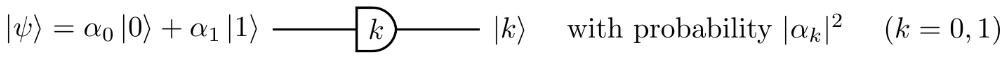
\includegraphics[width = 35em]{images/1.jpg}
\end{center}

In this process, the probability acquired by:$$
\begin{aligned}
|a_k|^2
    &= |\bk{k}{\psi}|^2\\
    &= \bk{\psi}{k}\bk{k}{\psi}\\
    &= \Bra{\psi}(\kb{k}{k})\Ket{\psi}\\
    &= \Bra{\psi} P_k\Ket{\psi}
\end{aligned},
$$ where $\kb{k}{k}$ is a projector. If it turns out that the measurement is $\Ket{k}$, then the original state $\Ket{\psi}$ is \textbf{irretrievably lost}. The sudden change from the pre-measurement state $\Ket{\psi}$ to post-measurement state $\Ket{0}$ or $\Ket{1}$ is called a \textbf{collapse} or \textbf{reduction}.
\end{remark}

\begin{remark}
Practically, this means that we describe measurement and observation with \underline{projectors} instead of \underline{unitary operators}.
\end{remark}

\section{The projection rule, and incomplete measurements}
\begin{proposition}[Any vector in $\HHH$ as the sum of the orthogonal projections onto the basis]\label{prop:projection-to-basis}
Suppose $\{e_k\}\subseteq \HHH$ is a basis. Then, any $\Ket{\psi}\in \HHH$ can be written as $$
\Ket{\psi} = \underset{k}{\sum} \alpha_k\Ket{e_k},
$$ so $$
\begin{aligned}
\Ket{\psi}
    &= (\mathbb{1}) \Ket{\psi}\\
    &= \prt{\underset{k}{\sum} \kb{e_k}{e_k}} \Ket{\psi}\\
    &= \underset{k}{\sum} \Ket{e_k}\bk{e_k}{\psi}\\
    &= \underset{k}{\sum} \alpha_k\Ket{e_k}
\end{aligned}
$$
\end{proposition}

\begin{remark}
A complete measurement represents the best we can do in terms of resolving state vectors in the basis states. But, we may not want measurement to distinguish all the elements of an orthonormal basis.
\end{remark}

\begin{example}\label{eg:incomp-meas}
A $4$-dimensional Hilbert space will have four distinct outcomes: $\Ket{e_1}, \Ket{e_2}, \Ket{e_3}$, and $\Ket{e_4}$, but we may only care about \textbf{distinguishing subspaces from each other}, not specific vectors (for instance, distinguishing only between $\{\Ket{e_1}, \Ket{e_2}\}$, $\{\Ket{e_3}, \Ket{e_4}\}$).
\end{example}

\begin{definition}[Incomplete Measurement]
Measurements as that which was shown in \ref{eg:incomp-meas} are known as incomplete measurements. Generally:
\begin{itemize}
    \item An incomplete measurement is \textbf{less informative} than complete measurements.
    \item An incomplete measurement is \textbf{less disruptive} than complete measurements.
\end{itemize}
\end{definition}

\begin{remark}
Generally, instead of \underline{projecting} on \underline{one-dimensional subspaces} spanned by vectors from an orthonormal basis (like that we have derived in proposition \ref{prop:projection-to-basis}), we can decompose the Hilbert space of interest into \textbf{mutually orthogonal subspaces of various dimensions} and \textbf{project onto them}.
\end{remark}

\noindent A full system of projectors satisfies two conditions:
\begin{itemize}
    \item (Orthogonality) $$
    P_kP_l = P_k\delta_{kl}.
    $$
    \item (Completeness) $$
    \underset{k}{\sum}P_k = 1
    $$
\end{itemize}

\noindent For any decomposition of identity into orthogonal projectors, by the completeness theorem, $\exists$ a measurement that takes a quantum system in $\Ket{\psi}$ and gives an output labelled $k$ with probability $$
\Bra{\psi} P_k\Ket{\psi}
$$ and leaves the system in $$
P_k\Ket{\psi}\text{, divided by the normalization factor.}
$$ That is: $$
\Ket{\psi} \mapsto \frac{P_k\Ket{\psi}}{\sqrt{\Bra{\psi} P_k\Ket{\psi}}}.
$$

\begin{example}[Example of an Incomplete Measurement]
Consider a $3$-dimensional Hilbert space $\HHH$, and its orthonormal basis $\{\Ket{e_1}, \Ket{e_2}, \Ket{e_3}\}$. Also, consider the two orthogonal projectors: $$
\begin{aligned}
P &= \Ket{e_1}\Bra{e_1} + \Ket{e_2}\Bra{e_2}\\
Q &= \Ket{e_3}\Bra{e_3}
\end{aligned}
$$

\noindent Firstly, they form a decomposition of the identity $$
P + Q = 1.
$$

\noindent Next, suppose we prepared a physical system in the state $$
\Ket{\psi} = \alpha_1 \Ket{e_1} + \alpha_2 \Ket{e_2} + \alpha_3 \Ket{e_3}.
$$ Then, a complete measurement will collapse it into a specific one of the three possible outcomes. However, an incomplete measurement does something different. It could, for instance, only differentiate between the subspaces associated with $P$ and $Q$. That is, the following are possible:
\begin{itemize}
    \item There is a probability of $\boxed{\Bra{\psi}P\Ket{\psi}} = |\alpha_1|^2 + |\alpha_2|^2$ to end up in a normalized vector $P\Ket{\psi}$, which means $$
    \Ket{\psi} \mapsto \frac{\alpha_1\Ket{e_1} + \alpha_2\Ket{e_2}}{\sqrt{|\alpha_1|^2 + |\alpha_2|^2}}.
    $$
    \item Alternatively, there is clearly a probability of $\boxed{\Bra{\psi}Q\Ket{\psi}} = |\alpha_3|^2$ to end up in a normalized vector $Q\Ket{\psi}$: $$
    \Ket{\psi} \mapsto \frac{\alpha_3\Ket{e_3}}{|\alpha_3|}.
    $$
\end{itemize}
\end{example}

\section{Observables}
\begin{definition}[Observables]
\textbf{Observables} are any \underline{measurable physical properties}, such as spin, position, momentum, and energy. For our purposes, we can also abstractly describe \textbf{observables} as \underline{any measurement in which \textbf{each term} has an \textbf{asso-}} \underline{\textbf{ciated numerical value}}.
\end{definition}

\noindent Let $\lambda_k$ be associated with each basis element $\Ket{e_k}$, then, the observable $$
A = \underset{k}{\sum}\lambda_k \kb{e_k}{e_k} = \lambda_k P_k,
$$ where $\lambda_k$ is an \textbf{eigenvalue} associated with the \textbf{eigenvector} $\Ket{e_k}$ or the \textbf{projector} $P_k$.

\begin{definition}[Recall]
We have seen the following types of operators:
\begin{itemize}
    \item (Unitary) $$
    A^\dag = A^{-1}
    $$
    \item (Normal) $$
    A^\dag A = AA^\dag
    $$
    \item (Hermitian) $$
    A^\dag = A
    $$
    \item (Positive semi-definite) $$
    \Bra{v}A \Ket{v} \geq 0, \forall \Ket{v}
    $$
\end{itemize}
\end{definition}

\begin{theorem}[Spectral Theorem]
An operator $A$ is \textbf{normal} $\iff$ $\exists$ unitary $U$ and diagonal $D$ such that $A = U^\dag D U$ (\textbf{unitarily diagnalizable}).
\end{theorem}
\begin{proof}(Sketch).
\begin{itemize}
    \item ($\implies$) If $A$ is normal, then we can associate a \underline{measurement} defined by:
    \begin{itemize}
        \item \textbf{Eigenvectors} of $A$, which is an orthonormal basis.
        \item \textbf{Eigenvalues} of $A$, which can be used to label the outcomes of the measurement.
    \end{itemize}

    If we choose the eigenvalues that are in $\RR$, $A$ becomes a Hermitian operator.

    [*Note: The standard measurement on a single qubit is often called the $Z$-measurement, because the Pauli $Z$-operator can be diagonalized in teh standard basis and be written as $$
    Z = (1)\kb{0}{0} + (-1)\kb{1}{1},
    $$ in which case the outcome states $\Ket{0}$ and $\Ket{1}$ are now written as $(1)$ and $(-1)$, respectively. We can similarly have the $X$- and $Y$-measurements defined by Pauli $X$ and $Y$ operators.]

    [**Note 2: Also, labels can be made into any symbols of your choice -- because we are talking about decomposition of the Hilbert space into mutually orthogonal subspaces that defines a \textbf{measurement}, not the \textbf{labels}. Because of this, we can WLOG make the labels real and make the operators Hermitian for our convenience.]

    Now, we incur theorem \ref{thm:condition-AB-is-commutative} for the rest of the proof to show that $A$ is indeed normal by showing $A, A^\dag$ are commutative.
    \item ($\impliedby$) $A = U^\dag D U$, then $A^\dag = U^\dag D^\dag (U^\dag)^\dag = U^\dag D^\dag U$. So, $$
    \begin{aligned}
    AA^\dag
        &= U^\dag D (UU^\dag) D^\dag U\\
        &= U^\dag D (UU^{-1}) D^\dag U\\
        &= U^\dag DD^\dag U\\
        &= U^\dag D^\dag D U\\
        &= U^\dag D^\dag (UU^{-1}) D U\\
        &= \prt{U^\dag D^\dag U}\prt{U^\dag D U}\\
        &= A^\dag A,
    \end{aligned}
    $$ simply by applying the properties of unitary and diagonal operators.
\end{itemize}
\end{proof}

\begin{definition}[Expected Value / Mean of $A$] \label{def:exp-A}
$$
\begin{aligned}
\langle A\rangle_{\Ket{\psi}} = \langle A\rangle
    &= \underset{k}{\sum}\lambda_k \Pr[k]\\
    &= \underset{k}{\sum}\lambda_k \Bra{\psi} (\kb{e_k}{e_k})\Ket{\psi}\\
    &= \Bra{\psi}\prt{\underset{k}{\sum}\lambda_k  \kb{e_k}{e_k}}\Ket{\psi}\\
    &= \Bra{\psi}A\Ket{\psi}.
\end{aligned}
$$

\noindent Notice how, when $A$ is a single projector, as in $A = \lambda_k\Ket{e_k}\Bra{e_k}$, then $\langle A\rangle$ is just the probability of the outcome associated with $A$.\\

\noindent [*Note: $\langle A\rangle$ is a shorthand that may be misleading, as it doesn't actually specify the $\Ket{\psi}$ that it depends on.]
\end{definition}

\noindent Next, we answer the question when is it true that operators $A,B$ are commutative: $$
AB = BA.
$$

\begin{definition}[\textbf{Eigenbasis}]
Say $\{\Ket{e_1}, \Ket{e_2}, \ldots, \Ket{e_n}\}$ is a basis of $A$. If its elements are also the eigenvectors of $A$, then we say it's the \textbf{eigenbasis} of $A$.
\end{definition}

\begin{theorem}\label{thm:condition-AB-is-commutative}
\hl{$AB = BA$ $\iff$ $A,B$ have the same eigenbasis (a.k.a. \textbf{simultaneously diagonalizable}).}
\end{theorem}

\begin{proof}
($\implies$) Consider the following derivation: Let $\Ket{e}$ be some eigenvector of $A$ with eigenvalue $\lambda$, $$
\begin{aligned}
AB 
    &= BA\\
\implies
AB\Ket{e}
    &= BA\Ket{e}\\
    &= B(\lambda\Ket{e})\\
    &= \lambda (B\Ket{e})
\end{aligned}.
$$ Note that this means that $B\Ket{e}$ is also an eigenvector of $A$ with eigenvalue of $\lambda$. Now, if $\lambda \neq 0$, then $B\Ket{e}$ is proportional to $\Ket{e}$, which is the same as saying that $\Ket{e}$ is an eigenvector of $B$. Since the choice of $\Ket{e}$ is arbitrary, this implies that the eigenbasis of $A$ and $B$ are the same. The reason why this is also called the \hl{simultaneously diagonalizable} is because: $\exists$ a basis in which both $A$ and $B$ are diagonal, i.e. any common eiganbasis of the two.\\

\noindent ($\impliedby$) Now, suppose $A,B$ share some eigenbasis, be it $\{\Ket{e_1}, \ldots, \Ket{e_n}\}$ (by definition, we can write $A\Ket{e_k} = \alpha_k \Ket{e_k}$ and $B\Ket{e_k} = \beta_k\Ket{e_k}$). Then, we can describe the beginning state $\Ket{\psi}$ in this basis as $$
\Ket{\psi} = \underset{k}{\sum}\lambda_k \Ket{e_k}.
$$
Then, $$
\begin{aligned}
(AB)\Ket{\psi}
    &= AB\prt{\underset{k}{\sum}\lambda_k \Ket{e_k}}\\
    &= \underset{k}{\sum}AB\lambda_k \Ket{e_k}\\
    &= \underset{k}{\sum}A\lambda_k \prt{B\Ket{e_k}}\text{, commute because $\lambda_k\in \CC$}\\
    &= \underset{k}{\sum}A\lambda_k \prt{\beta_k\Ket{e_k}} = \underset{k}{\sum}A\lambda_k \beta_k\Ket{e_k}\\
    &= \underset{k}{\sum}\lambda_k \beta_k(A\Ket{e_k})\text{, commute because $\lambda_k, \beta_k\in \CC$}\\
    &= \underset{k}{\sum}\lambda_k \beta_k(\alpha_k\Ket{e_k})\\
    &= \underset{k}{\sum}\lambda_k \beta_k\alpha_k\Ket{e_k}
\end{aligned}.
$$ Now, it is clear that you can get the same form: $\underset{k}{\sum}\lambda_k \beta_k\alpha_k\Ket{e_k}$ from $(BA)\Ket{\psi}$ since now all the elements in there are commutative. So, clearly, $$
(AB)\Ket{\psi} = (BA)\Ket{\psi}\text{ for arbitrary }\Ket{\psi}\implies AB = BA
$$
\end{proof}

\begin{definition}[Compatible]\label{def:compatibility}
Based off of the discussion in theorem \ref{thm:condition-AB-is-commutative}, we define operators $A,B$ that are commutative to be \textbf{compatible}; otherwise, they are \textbf{incompatible}.
\end{definition}

\begin{remark}
What does definition \ref{def:compatibility} tell us in terms of measurements?
\begin{itemize}
    \item If $A,B$ as observables are compatible. Then, the order of measuring them won't matter.
    \item However, if they are incompatible, say one is position and one is momentum, then measuring them in one order or another would lead to different numerical values of observations.
\end{itemize}
\end{remark}

\subsection{Uncertainty Principle}
This is really an application of theorem \ref{thm:condition-AB-is-commutative} and definition \ref{def:compatibility}.\\

\noindent Consider a very large system that we prepared, which started in the initial state of $\Ket{\psi}$. Now, we measure the observable $A$ on half of the qubits and $B$ on the other half. Then, we can calculate:
\begin{itemize}
    \item $\langle A\rangle$ and $\langle B\rangle$, and
    \item $\sigma_A$ and $\sigma_B$ which are the standard deviations from the expected values.
\end{itemize}

\noindent If $A,B$ are \textbf{compatible}, we can make $\sigma_A = \sigma_B = 0$, simultaneously. However, what's interesting is when $A,B$ are \textbf{incompatible}.

\begin{theorem}[Uncertainty Principle]
The uncertainty principle for operators $A,B$ states that: $$
\boxed{\sigma_A\sigma_B \geq \left| \frac{1}{2i}\langle [A,B] \rangle \right|},
$$ where $[A,B] = AB - BA$ is the \textbf{commutator}.
\end{theorem}

\begin{example}[Heisenberg's Uncertainty Principle]
It can be shown that, if we consider $A,B$ to be position and momentum, then $\left|\frac{1}{i}\langle [x,p] \rangle\right| = \hbar$, so $$
\sigma_x \sigma_p \geq \frac{\hbar}{2}
$$
\end{example}

\begin{remark}
One more thing to notice is the following. Suppose we instead have three operators, $A,B,C$. We start with some state in $A$, denoted $\Ket{a}$, and want to output $\Ket{c}\in C$. What are the probabilities? Well, there are two ways:
\begin{itemize}
    \item We sum over the intermediate steps (that is probability to get to $b_k$ from $a$, and then probability to get to $c$ from $b$): $$
    \Pr[c] = \underset{k}{\sum} |\bk{a}{b_k}|^2|\bk{b_k}{c}|^2
    $$
    \item We directly compute the probability:$$
    \begin{aligned}
    \Pr[c]
        &= |\bk{c}{a}|^2\\
        &= \left|\underset{k}{\sum}\Bra{c}\kb{b_k}{b_k}\Ket{a}\right|^2\text{, because $\underset{k}{\sum}\kb{b_k}{b_k}$ = 1}\\
    \end{aligned}
    $$
\end{itemize}

\noindent But, notice that, in general, $$
\left|\underset{k}{\sum}\Bra{c}\kb{b_k}{b_k}\Ket{a}\right|^2\neq \underset{k}{\sum} |\bk{a}{b_k}|^2|\bk{b_k}{c}|^2,
$$ unless $[A,B] = 0$ or $[B,C] = 0$ (should be easy to verify by direct computation). \hl{This is same as saying, $\iff$ $A$ and $B$ or $B$ and $C$ are comparable}.
\end{remark}

\end{document}